\subsection{Sensor DHT22}

El sensor DHT22 mide temperatura y humedad. Se conecta de la siguiente manera:
\begin{figure}[!ht]
    \centering
    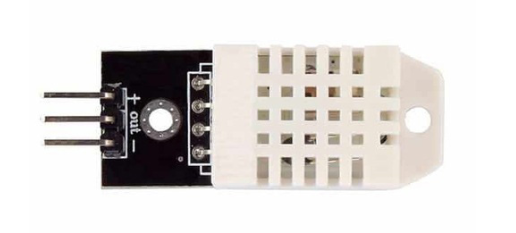
\includegraphics[width=0.4\textwidth]{assets/metodos_herramientas/dht22.png}
    \caption{Sensor DHT22.}
    \label{fig:dht22}
\end{figure}
\begin{itemize}
    \item VCC a 3.3--6 V.
    \item OUT a un pin digital con protocolo 1-wire.
    \item GND a tierra.
\end{itemize}

\begin{figure}[!ht]
    \centering
    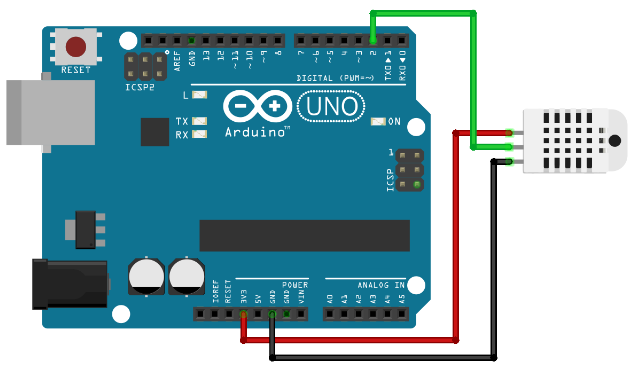
\includegraphics[width=0.5\textwidth]{assets/metodos_herramientas/arduino_dht22.png}
    \caption{Conexión del sensor DHT22 a Arduino.}
    \label{fig:arduino_dht22}
\end{figure}

\paragraph{Herramientas de software}
\begin{itemize}
    \item Arduino IDE 2.2.1 en Windows 10.
    \item Librerías de Adafruit: \texttt{DHT sensor library} y \texttt{Adafruit Unified Sensor}.
\end{itemize}

\subsection{Celda de carga y módulo HX711}
Las celdas de carga son los sensores que recolectan información sobre el peso de una carga aplicada sobre los mismos. Los sensores a utilizar son equivalentes a los de la ilustración 3, cuentan con 4 cables y 4 orificios roscados para fijar la celda, así como una imagen indicativa de la dirección de la carga.

\begin{figure}[!ht]
    \centering
    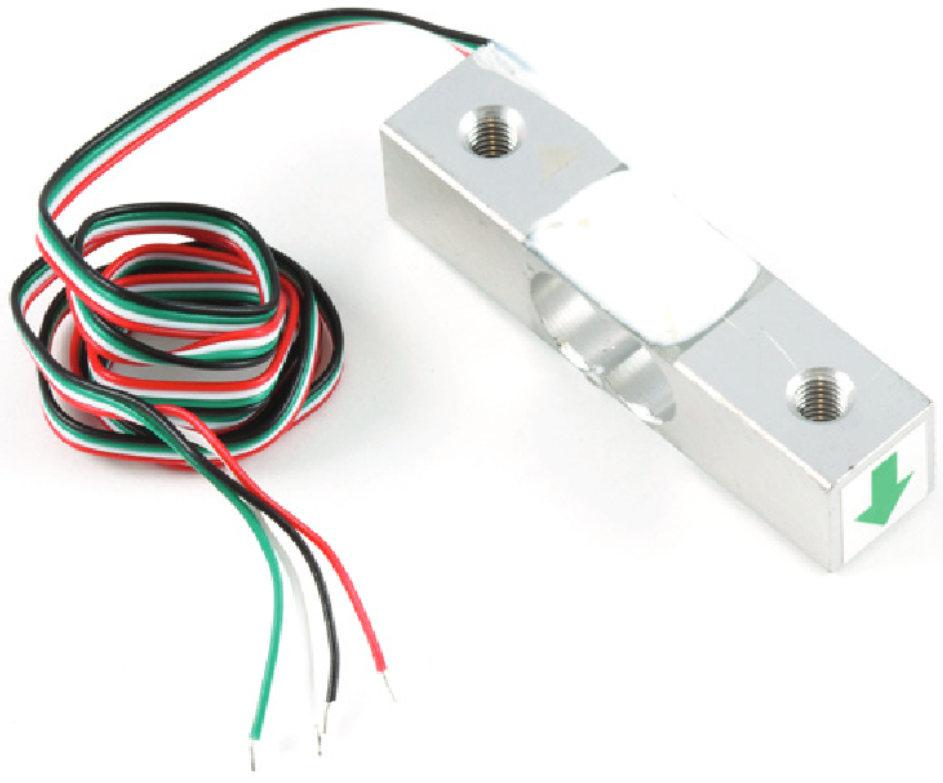
\includegraphics[width=0.5\textwidth]{assets/metodos_herramientas/celda_carga.png}
    \caption{Celda de carga.}
    \label{fig:celda_carga}
\end{figure}
\newpage

El módulo HX711 es una placa electrónica que funciona como interfaz entre una placa Arduino y una celda de carga. Este se muestra en la ilustración \ref{fig:hx711}. El módulo HX711 es un convertidor analógico a digital (ADC) de 24 bits, diseñado específicamente para aplicaciones de pesaje y medición de fuerza. Permite leer las señales analógicas de la celda de carga y convertirlas en valores digitales que pueden ser procesados por un microcontrolador como Arduino.

\begin{figure}[!ht]
    \centering
    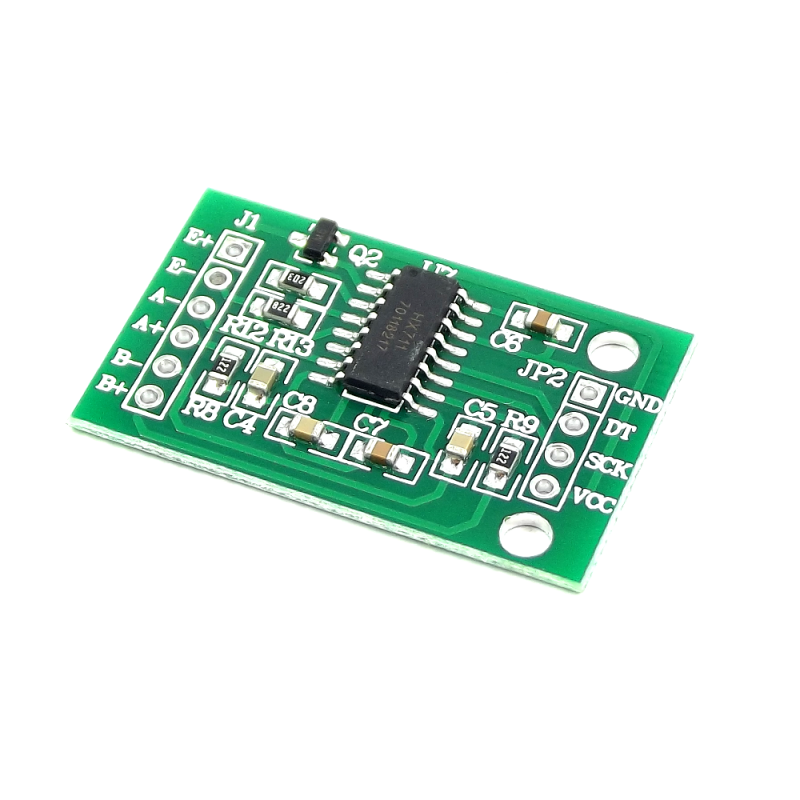
\includegraphics[width=0.5\textwidth]{assets/metodos_herramientas/hx711.png}
    \caption{Módulo HX711.}
    \label{fig:hx711}
\end{figure}
Las conexiones se realizan de acuerdo a las tablas \ref{tab:conexiones_celda_hx711} y \ref{tab:conexiones_hx711_arduino}. La celda de carga se conecta al módulo HX711, y este último se conecta a la placa Arduino. El módulo HX711 requiere una alimentación de 5 V y tiene dos pines de salida: uno para la señal de datos (DT) y otro para el reloj (SCK).
\begin{table}[!ht]
    \centering
    \rowcolors{2}{gray!10}{white}
    \begin{tabularx}{\textwidth}{>{\bfseries}X X}
        \toprule
        \textbf{COLOR DEL CABLE} & \textbf{CONECCIÓN EN MÓDULO} \\
        \midrule
        ROJO                     & E+                           \\
        NEGRO                    & E-                           \\
        BLANCO                   & A-                           \\
        VERDE                    & A+                           \\
        \bottomrule
    \end{tabularx}
    \caption{\textit{conexiones celda-HX711}}
\end{table}
\begin{table}[!ht]
    \centering
    \rowcolors{2}{gray!10}{white}
    \begin{tabularx}{\textwidth}{>{\bfseries}X X}
        \toprule
        \textbf{PIN HX711} & \textbf{CONECCIÓN EN ARDUINO} \\
        \midrule
        GND                & GND                           \\
        DT                 & A1                            \\
        SCK                & A0                            \\
        VCC                & 5 V                           \\
        \bottomrule
    \end{tabularx}
    \caption{\textit{conexiones HX711-Arduino}}
\end{table}
\newpage

\paragraph{Ejemplo de código HX711}\mbox{}

\begin{lstlisting}[language=C++, caption={Ejemplo de código HX711}, label={lst:ejemplo_hx711}]
#include "HX711.h"
const int DOUT = A1;
const int CLK = A0;
HX711 balanza;

void setup() {
  Serial.begin(9600);
  balanza.begin(DOUT, CLK);
  balanza.set_scale(439430.25);
  balanza.tare();
}

void loop() {
  Serial.println(balanza.get_units());
  delay(1000);
}
\end{lstlisting}

\subsection{Controlador ESP32}
El ESP32 integra Wi-Fi y Bluetooth en un solo chip con bajo consumo en modo Deep Sleep (~10 \textmu{}A a 3.3 V).
\begin{itemize}
    \item Procesador: Xtensa LX6, 32 bits, hasta 240 MHz.
    \item RAM: 520 KB SRAM.
\end{itemize}

Para utilizar el controlador con el Arduino IDE2.0 es necesario agregar el siguiente paquete a Additional Boards Manager como se muestra en la figura  \ref{fig:arduino_placas} y el código \ref{lst:esp32_boards_manager}.
\begin{lstlisting}[language=, label={lst:esp32_boards_manager}, caption={URL para Boards Manager de ESP32}]
https://raw.githubusercontent.com/espressif/arduino-esp32/gh-pages/package_esp32_index.json
\end{lstlisting}

\newpage

\begin{figure}[!ht]
    \centering
    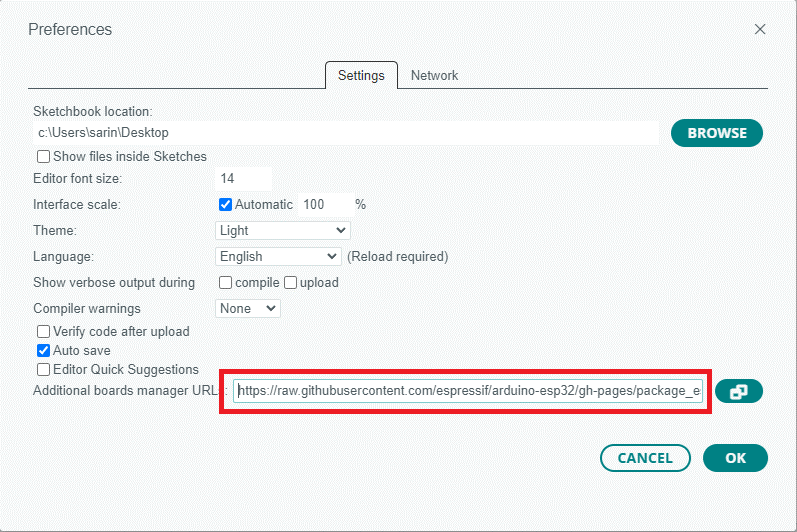
\includegraphics[width=0.75\textwidth]{assets/metodos_herramientas/arduino_placas.png}
    \caption{Selección de placas ESP32 en Arduino IDE.}
    \label{fig:arduino_placas}
\end{figure}

El siguiente paso es instalar los controladores para la placa ESP32, se muestra en la figura  \ref{fig:arduino_install_esp32}.

\begin{figure}[!ht]
    \centering
    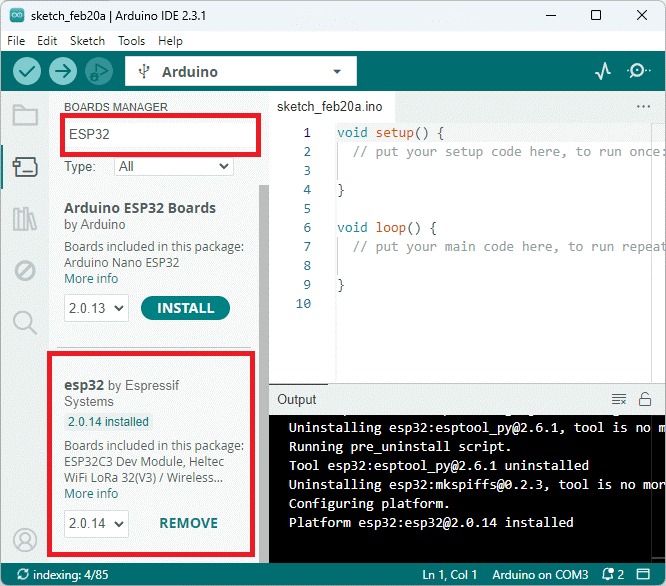
\includegraphics[width=0.75\textwidth]{assets/metodos_herramientas/arduino_install_esp32.png}
    \caption{Instalación del soporte para ESP32 en Arduino IDE.}
    \label{fig:arduino_install_esp32}
\end{figure}

\newpage

Código de prueba:
\begin{lstlisting}[language=C++, label={lst:esp32_blink}, caption={Ejemplo de código de parpadeo de LED en ESP32}]
#include <Arduino.h>
#define LED 2
void setup() {
  Serial.begin(115200);
  pinMode(LED, OUTPUT);
}
void loop() {
  digitalWrite(LED, HIGH);
  delay(1000);
  digitalWrite(LED, LOW);
  delay(1000);
}
\end{lstlisting}

\subsection{Micrófono INMP441}
\begin{figure}[!ht]
    \centering
    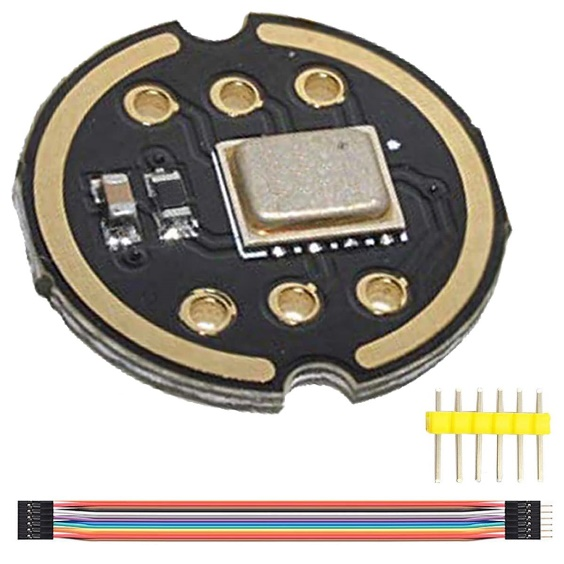
\includegraphics[width=0.75\textwidth]{assets/metodos_herramientas/inmp441.png}
    \caption{Módulo de micrófono INMP441.}
    \label{fig:inmp441}
\end{figure}

El sensor INMP441 es un micrófono multidireccional que utiliza el protocolo I2S~\cite{keysight_i2s_blog} para transferencia de audio, de la misma manera que, y como se mencionó en los trabajos relacionados, el dispositivo INMP401 es utilizado con el controlador ESP8266, el dispositivo INMP441 es comúnmente utilizado con el dispositivo ESP32, principalmente por su compatibilidad mediante el protocolo I2S. El módulo INMP441 se muestra en la figura  7~\cite{inmp441_datasheet}.
